\documentclass[tikz,border=4pt]{standalone}
% Shared visual grammar: role fills, dark connectors, and 7-point typography.
% Build each standalone figure from this directory. No external images required.
\pdfinfoomitdate=1
\pdftrailerid{}
\usepackage[T1]{fontenc}
\usepackage{helvet}
\renewcommand{\familydefault}{\sfdefault}
\usepackage{amsmath,amssymb}
\hyphenpenalty=10000
\exhyphenpenalty=10000
\usetikzlibrary{arrows.meta,calc,fit,positioning,decorations.pathreplacing,backgrounds}
\definecolor{ink}{HTML}{172B3A}
\definecolor{muted}{HTML}{586D85}
\definecolor{datafill}{HTML}{F1F5F9}
\definecolor{dataline}{HTML}{62748E}
\definecolor{modelfill}{HTML}{E5E9FF}
\definecolor{modelline}{HTML}{7887C7}
\definecolor{llmfill}{HTML}{FFE4E8}
\definecolor{llmline}{HTML}{E68494}
\definecolor{truthfill}{HTML}{D0FAE5}
\definecolor{truthline}{HTML}{35A782}
\newcommand{\seven}{\fontsize{7}{8.5}\selectfont}
\tikzset{
 every node/.append style={font=\seven,text=ink,align=center},
 box/.style={draw=dataline,fill=white,rounded corners=3pt,line width=.65pt,inner sep=5pt,minimum height=8mm},
 data/.style={box,fill=datafill},
 model/.style={box,draw=modelline,fill=modelfill},
 llm/.style={box,draw=llmline,fill=llmfill},
 truth/.style={box,draw=truthline,fill=truthfill},
 title/.style={font=\seven\bfseries,inner sep=1pt},
 word/.style={text=muted,inner sep=1pt,align=center},
 label/.style={fill=white,inner xsep=2pt,inner ysep=1pt,text=muted},
 flow/.style={-{Stealth[length=2.4mm,width=1.9mm]},draw=ink,line width=1.2pt,shorten >=1.5pt},
 branch/.style={-{Stealth[length=2mm,width=1.6mm]},draw=ink,line width=.9pt,shorten >=1pt},
 route/.style={draw=ink,line width=1.2pt},
 update/.style={-{Stealth[length=2.2mm,width=1.7mm]},draw=modelline,line width=1pt,dash pattern=on 3pt off 2pt,shorten >=1.5pt},
 boundary/.style={draw=dataline,dash pattern=on 3pt off 2pt,rounded corners=3pt,line width=.6pt},
 chip/.style={minimum height=4mm,inner xsep=3pt,inner ysep=1.5pt,rounded corners=2pt},
}
% Optional role key. Anchor at the center of an uncluttered final row.
\newcommand{\rolekey}[2]{
 \node[word,anchor=east] at (#1-6.6,#2) {\textit{Key}};
 \node[data,chip] at (#1-5.2,#2) {records / data};
 \node[model,chip] at (#1-1.9,#2) {learned model / policy};
 \node[llm,chip] at (#1+1.65,#2) {LLM signal};
 \node[truth,chip] at (#1+4.95,#2) {labels / evaluation};
}

\begin{document}
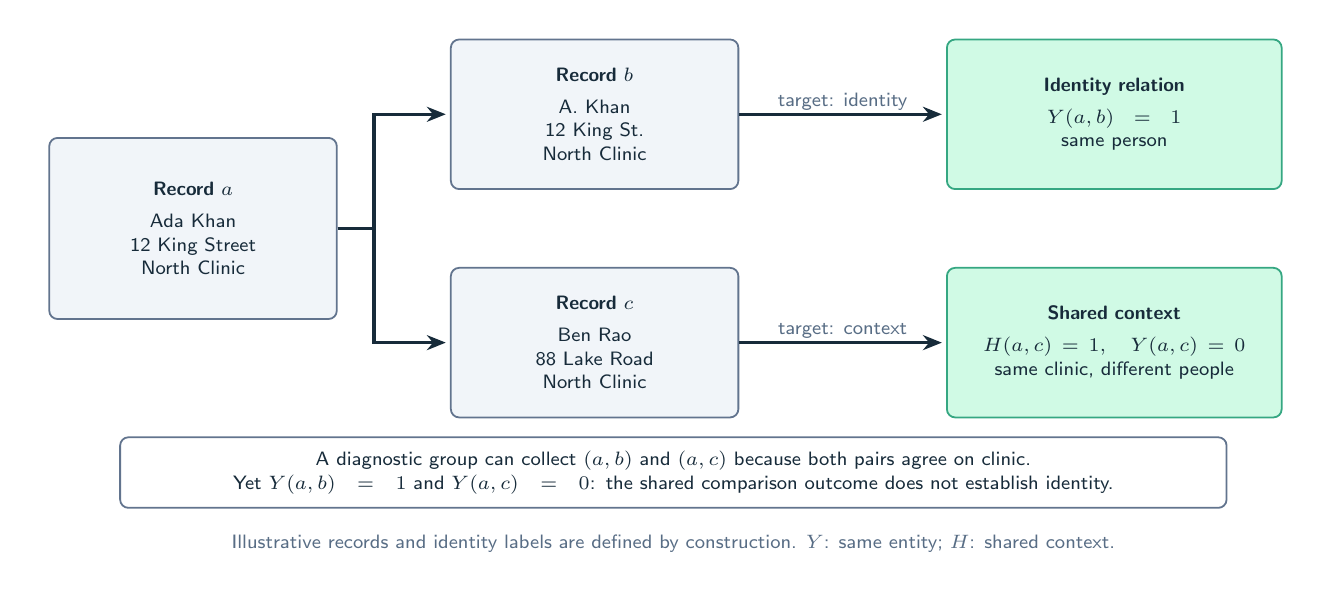
\begin{tikzpicture}

\useasboundingbox (-.2,.3) rectangle (16.1,-6.55);
\node[data,text width=33mm,minimum height=23mm] (a) at (1.9,-2.25) {\textbf{Record $a$}\\[3pt]Ada Khan\\12 King Street\\North Clinic};
\node[data,text width=33mm,minimum height=19mm] (b) at (7,-.8) {\textbf{Record $b$}\\[3pt]A. Khan\\12 King St.\\North Clinic};
\node[data,text width=33mm,minimum height=19mm] (c) at (7,-3.7) {\textbf{Record $c$}\\[3pt]Ben Rao\\88 Lake Road\\North Clinic};
\node[truth,text width=39mm,minimum height=19mm] (id) at (13.6,-.8) {\textbf{Identity relation}\\[3pt]$Y(a,b)=1$\\same person};
\node[truth,text width=39mm,minimum height=19mm] (topic) at (13.6,-3.7) {\textbf{Shared context}\\[3pt]$H(a,c)=1,\quad Y(a,c)=0$\\same clinic, different people};
\draw[flow] (a.east) -- (4.2,-2.25) |- (b.west);
\draw[flow] (a.east) -- (4.2,-2.25) |- (c.west);
\draw[flow] (b.east) -- node[label,above] {target: identity} (id.west);
\draw[flow] (c.east) -- node[label,above] {target: context} (topic.west);
\node[box,text width=137mm] at (8,-5.35) {A diagnostic group can collect $(a,b)$ and $(a,c)$ because both pairs agree on clinic.\\Yet $Y(a,b)=1$ and $Y(a,c)=0$: the shared comparison outcome does not establish identity.};
\node[word] at (8,-6.25) {Illustrative records and identity labels are defined by construction. $Y$: same entity; $H$: shared context.};

\end{tikzpicture}
\end{document}
